\section{Einführung}\label{sec:introduction}
\IEEEPARstart{S}ysteme zur Spracherkennung finden eine zunehmende Verbreitung und Beliebtheit in unserem alltäglichen Leben.
Sie ermöglichen multimodale Interaktionen oder auch reine Voice Interfaces \cite{Harris.2004}.
Das Anwendungsspektrum reicht von sprachgesteuerten Smarthome-Systemen über Smartphones hin zum Einsatz in Autos \cite{Yu.2014}.
Bei weltweit über 7000 gesprochenen Sprachen ist es nur konsequent, multilinguale Spracherkennungssysteme zu entwickeln \cite{Gary.2018}.
Eingesetzt werden diese bei Situationen, in denen die Sprache des Sprechers nicht bekannt oder für eine Sprache nur wenig
Trainingsdaten vorhanden sind. In solch einem Fall kann die gemeinsame Nutzung von Phonemen, die fehlenden Daten ausgleichen [fehlt noch].
Ein Phonem ist eine abstrakte Repräsentation aller Laute einer Sprache \citation{Zissman.2001}.
Der nachfolgende Abschnitt beschreibt die einzelnen Komponenten eines multilingualen Spracherkennungssystems.
Die darauffolgenden Kapitel analysieren die heutzutage dafür eingesetzten Verfahren.
Im Fokus stehen Deep Neural Networks, wie dessen Modelle trainiert werden und welche Probleme es dabei gibt.

\subsection{Pipeline}
Die Abbildung \ref{fig:pipeline} zeigt die Komponenten, aus dem ein multilinguales Spracherkennungssystem besteht.
Am Anfang steht ein analoges Audiosignal das digitalisiert wird. Aus diesen Daten werden aus kleinen Sequenzen
Feature-Vektoren extrahiert. In Abbildung \ref{fig:pipeline} ist als Beispielausgabe für diesen Teilschritt ein Spektrogramm dargestellt – bei dem die einzelnen Frequenzen bildlich dargestellt werden.
Die Feature-Vektoren müssen so gewählt werden, dass die kleinste effizienteste Menge für die Sprachverarbeitung
entsteht und unnötige Informationen bereits vor dem Decoder herausgefiltert werden.
Die gewonnenen Feature-Vektoren werden als Eingabe für die Sprachidentifikation genutzt. Die Information
über die identifizierte Sprache kombiniert mit den Feature-Vektoren bilden die Eingabe für den Decoder. Der Decoder bildet aus dieser Eingabe,
dem Akkustik-, Sprach- und Lexikalmodell den gesprochenen Text. Die drei Modelle werden von \cite{Tom.2016} wie folgt beschrieben:

\begin{itemize}
    \item \textit{Akkustikmodell.} Die gesprochene Sprache wird abgebildet durch einzelne Phoneme.
    \item \textit{Lexikalmodell.} Alle gültigen Wörter einer Sprache.
    \item \textit{Sprachmodell.} Die Wahrscheinlichkeit für einen syntaktisch und semantisch korrekten Satz.
            Beispielsweise folgt auf das englische Wort \glqq{thank}\grqq{} mit einer sehr hohen Wahrscheinlichkeit das Wort \glqq{you}\grqq{} oder
        \glqq{god}\grqq{}.
\end{itemize}

\begin{figure}[h!]
    \centering
    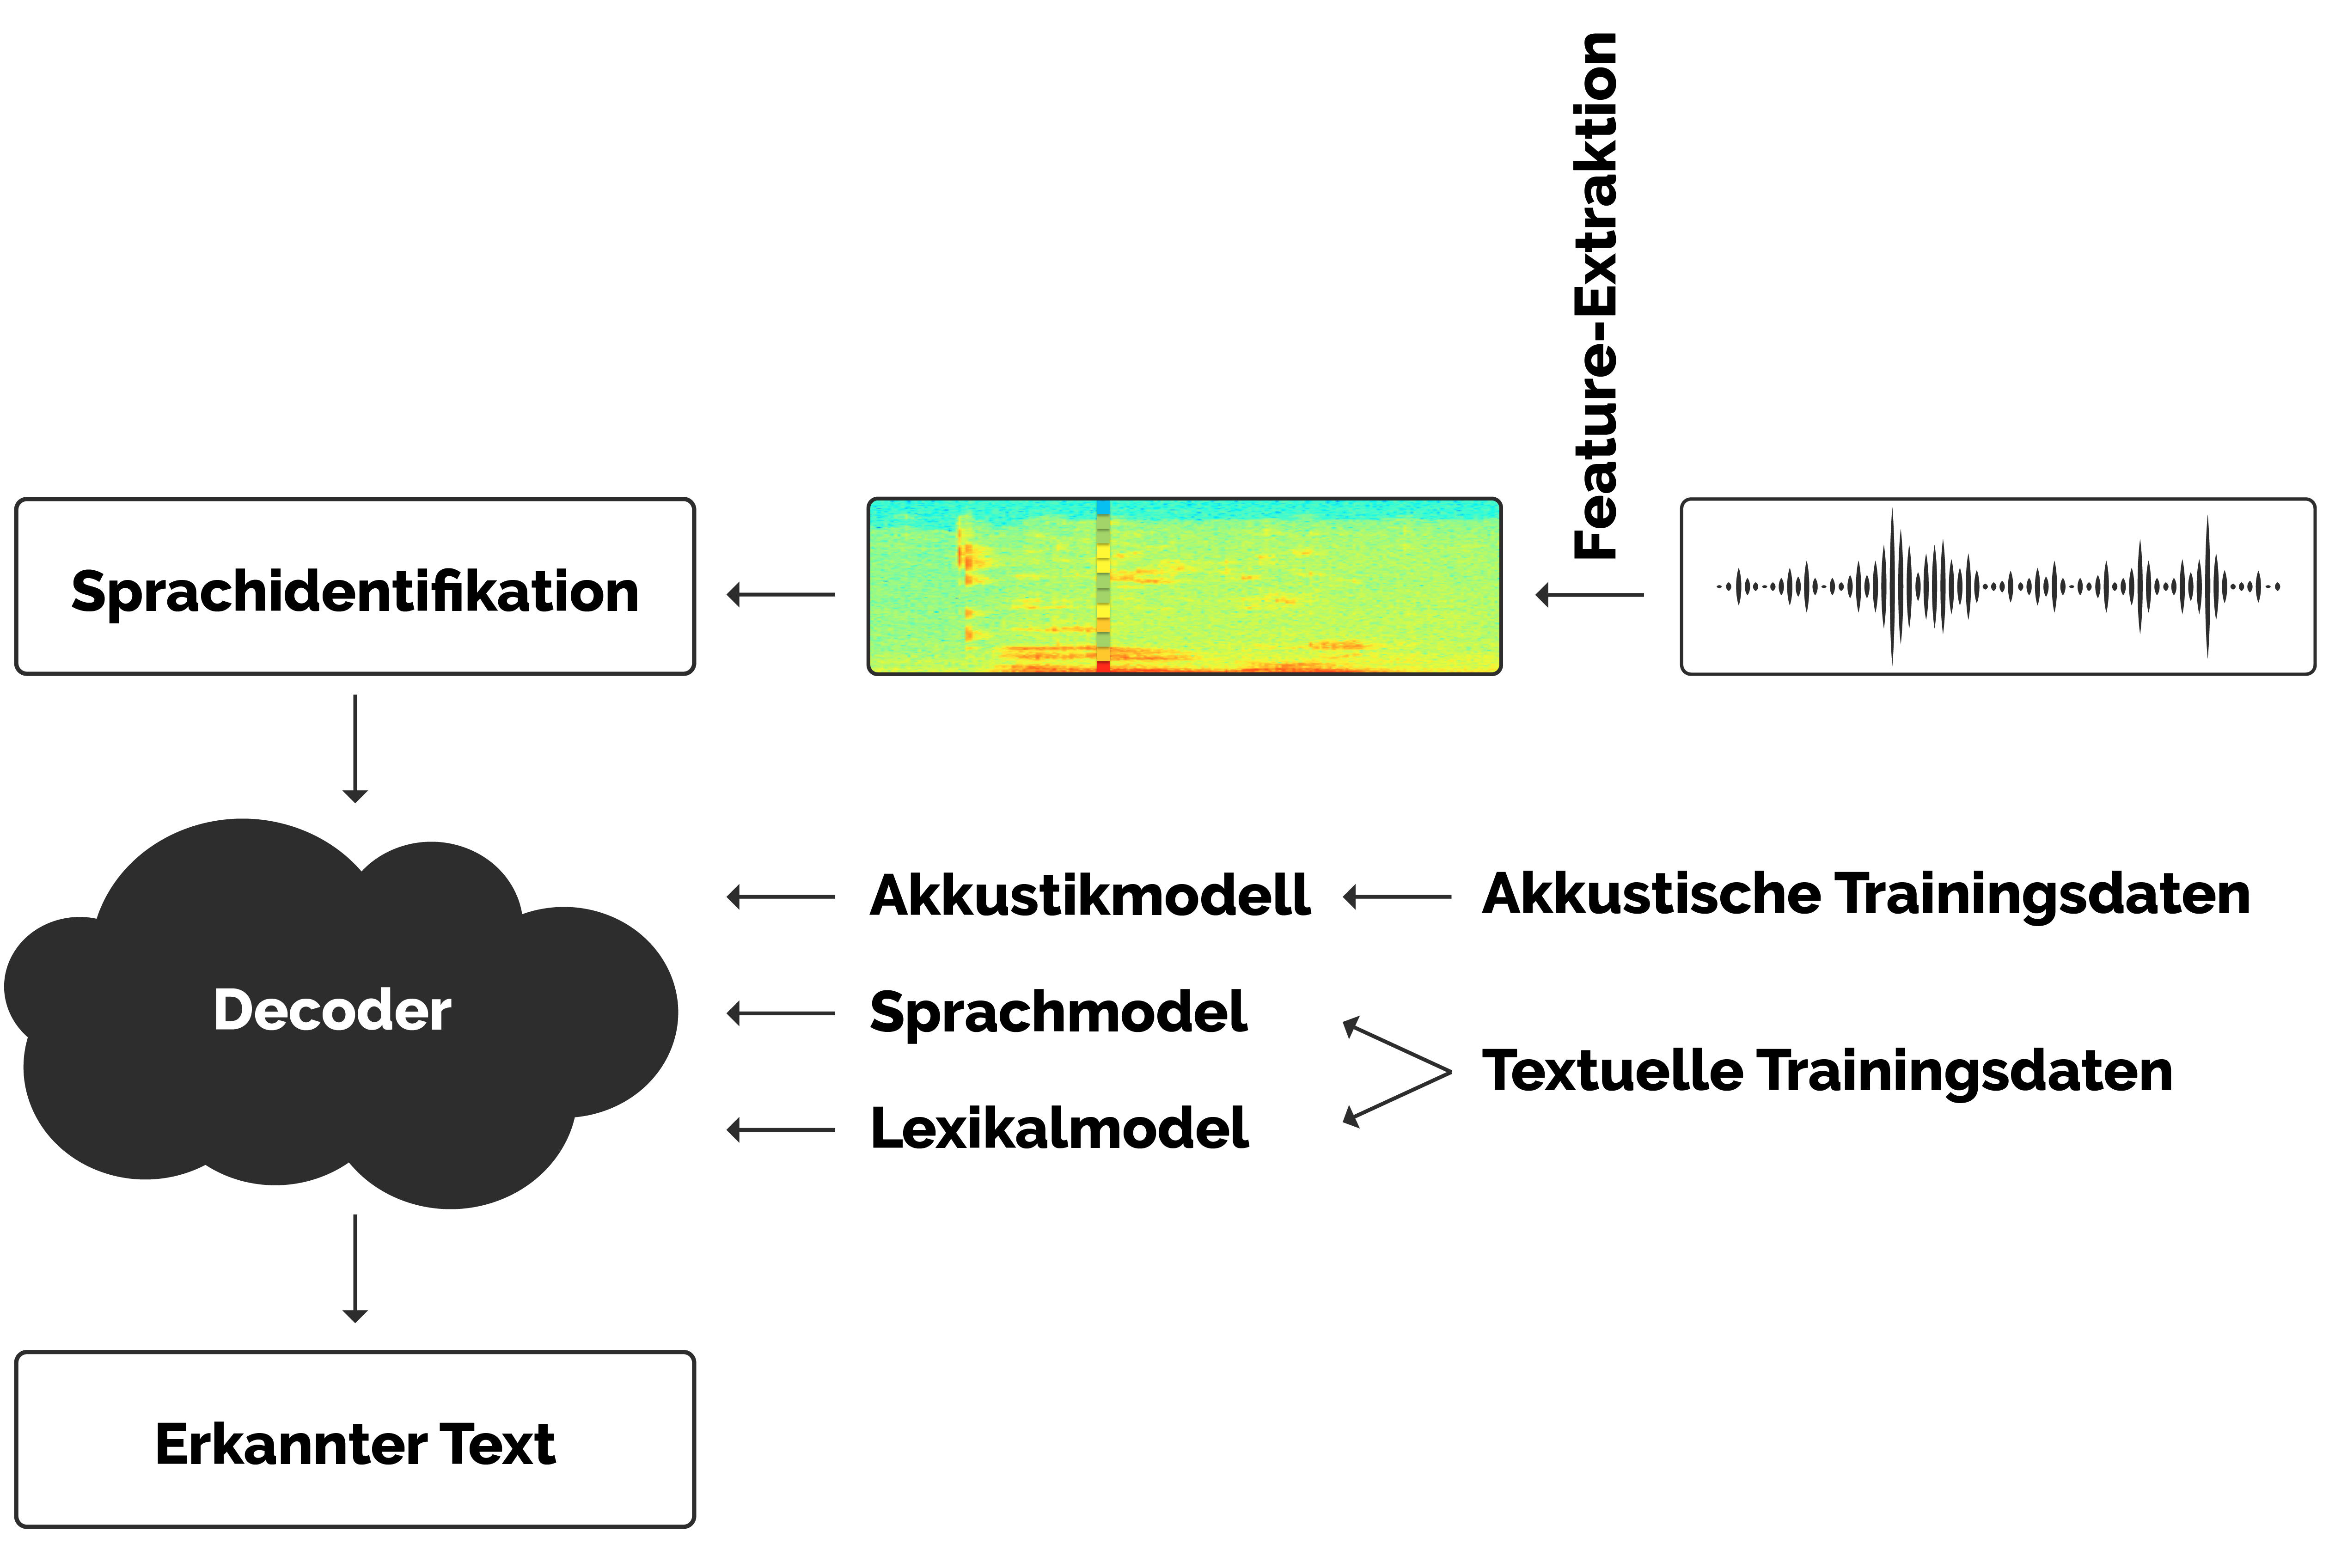
\includegraphics[width=1\linewidth]{images/pipeline}
    \caption{Pipeline eines Spracherkennungssystems (Eigene Darstellung, in Anlehnung an: \cite{Tom.2016}) }%\cite{??}}
    \label{fig:pipeline}
\end{figure}

Die Trainingsdaten für die beschriebenen Modelle werden in die folgenden zwei Gruppen unterteilt \cite{Tom.2016}:

\begin{itemize}
    \item \textit{Akkustische Trainingsdaten.} Diese Daten werden genutzt um das Eingangssignal auf Phoneme abzubilden.
    \item \textit{Textuelle Trainingsdaten.} Bilden Grammatik und semantische Informationen in den Modellen ab.
\end{itemize}

